\documentclass[aspectratio=169]{beamer}

% Pacotes essenciais
\usepackage[utf8]{inputenc}
\usepackage[T1]{fontenc}
\usepackage[brazilian]{babel}
\usepackage{graphicx}
\usepackage{tikz}
\usepackage{booktabs}
\usepackage{array}
\usepackage{colortbl}

% Fonte moderna Roboto
\usepackage[sfdefault]{roboto}
\usepackage[T1]{fontenc}

% Definição das cores
\definecolor{vermelhoPrincipal}{HTML}{b11116}
\definecolor{azulComplementar}{HTML}{3a5461}
\definecolor{brancoFundo}{HTML}{FFFFFF}
\definecolor{cinzaClaro}{HTML}{F4F4F4}

% Configuração do tema
\usetheme{Madrid}
\usecolortheme{default}

% Cores personalizadas - texto sempre em preto
\setbeamercolor{structure}{fg=black}
\setbeamercolor{palette primary}{bg=vermelhoPrincipal,fg=white}
\setbeamercolor{palette secondary}{bg=azulComplementar,fg=white}
\setbeamercolor{palette tertiary}{bg=vermelhoPrincipal,fg=white}
\setbeamercolor{palette quaternary}{bg=azulComplementar,fg=white}
\setbeamercolor{frametitle}{bg=vermelhoPrincipal,fg=white}
\setbeamercolor{background canvas}{bg=brancoFundo}
\setbeamercolor{title}{fg=black}
\setbeamercolor{subtitle}{fg=azulComplementar}
\setbeamercolor{author}{fg=black}
\setbeamercolor{date}{fg=black}
\setbeamercolor{itemize item}{fg=black}
\setbeamercolor{itemize subitem}{fg=black}
\setbeamercolor{enumerate item}{fg=black}
\setbeamercolor{block title}{bg=vermelhoPrincipal,fg=white}
\setbeamercolor{block body}{bg=vermelhoPrincipal!10,fg=black}
\setbeamercolor{normal text}{fg=black}

% Configurar fonte dos itemize
\setbeamerfont{itemize/enumerate body}{size=\scriptsize}
\setbeamerfont{itemize/enumerate subbody}{size=\scriptsize}

% Marcadores modernos e minimalistas
\setbeamertemplate{itemize item}{\raisebox{0.2ex}{\rule{0.6ex}{0.6ex}}}
\setbeamertemplate{itemize subitem}{\raisebox{0.3ex}{\rule{0.4ex}{0.4ex}}}
\setbeamertemplate{itemize subsubitem}{\raisebox{0.35ex}{\rule{0.3ex}{0.3ex}}}
\setbeamertemplate{enumerate items}[square]

% Transições suaves
\setbeamercovered{transparent}

% Remover símbolos de navegação
\setbeamertemplate{navigation symbols}{}

% Customizar o cabeçalho com barra vermelha e logo
\setbeamertemplate{headline}{
  \begin{beamercolorbox}[wd=\paperwidth,ht=0.6cm,dp=0.15cm,leftskip=0.2cm,rightskip=0.4cm]{palette primary}
    \raisebox{-0.05cm}{
\includegraphics[height=0.45cm]{imgs/base/fatec-rgt.png}}
    \hfill
    \raisebox{-0.18cm}{
\includegraphics[height=0.85cm]{imgs/base/governo-sp-secretaria-logo.png}}
    \hspace{0.2cm}
    \raisebox{-0.08cm}{
\includegraphics[height=0.6cm]{imgs/base/cps-logo.png}}
  \end{beamercolorbox}
}
% Remover sombras dos blocks
\setbeamertemplate{blocks}[default]
\setbeamertemplate{itemize/enumerate body begin}{\scriptsize}
\setbeamertemplate{itemize/enumerate subbody begin}{\scriptsize}
% Customizar o rodapé
\setbeamertemplate{footline}{
  \begin{beamercolorbox}[wd=\paperwidth,ht=0.4cm,dp=0.2cm,leftskip=0.3cm,rightskip=0.3cm]{palette secondary}
    \usebeamerfont{footline}
    \insertshortauthor \hfill \hfill {\fontsize{5}{6}\selectfont\insertshorttitle} \hfill \hfill \insertframenumber/\inserttotalframenumber
  \end{beamercolorbox}
}

% Customizar título do frame
\setbeamertemplate{frametitle}{
  \vspace{0.3cm}
  \textcolor{black}{\insertframetitle}
  \vspace{0.1cm}
}

% Informações da apresentação
\title{Identificação do Ácaro Varroa em Abelhas \\ Apis Mellifera por
Meio de Inteligência Artificial}
\subtitle{}
\author[DSM]{LANNA, G.; ARAUJO, I.; KUSAKA, J.; BELARMINO, Y.}
\institute{Desenvolvimento de Software Multiplataforma\\FATEC Registro}
\date{\today}

\begin{document}

% ─── SLIDE 1 — TÍTULO (original) ─────────────────────────────────────────────
\begin{frame}
  \vspace{0.8cm}
  \begin{center}
    \begin{tikzpicture}
      \draw[vermelhoPrincipal, line width=2pt] (-4,0) -- (4,0);
    \end{tikzpicture}
    
    \vspace{0.4cm}
    
    {\normalsize\bfseries\inserttitle}\par
    
    \vspace{0.2cm}
    
    {\tiny\insertauthor}\par
    
    \vspace{0.1cm}
    
    {\small\textcolor{azulComplementar}{\insertsubtitle}}\par
    
    \vspace{0.5cm}
    
    \begin{tikzpicture}
      \draw[azulComplementar, line width=1.5pt] (-2.5,0) -- (2.5,0);
    \end{tikzpicture}
    
    \vspace{0.3cm}
    
    {\scriptsize\insertinstitute}\par
    
    \vspace{0.01cm}
    
    {\tiny\textcolor{azulComplementar}{\insertdate}}\par
  \end{center}
\end{frame}

% ─── SLIDE 2 — AGENDA (original) ─────────────────────────────────────────────
\begin{frame}[b]{Agenda}
  \begin{itemize}
    \item Pitch
    \item Problematização
    \item Estado da Arte
    \item Objetivo
    \item Ferramental
    \item Metodologia
    \item Apresentação prática
    \item Resultados e Discussões
  \end{itemize}
  
  \vfill
  
  \hfill{\scriptsize \textbf{Duração:} 10 a 11 min.}
\end{frame}

% ─── PITCH ───────────────────────────────────────────────────────────────────
\section{Pitch}

\begin{frame}[b]{Pitch}
  \begin{columns}[T]
    \begin{column}{0.58\textwidth}
      \begin{itemize}
        \item O \textbf{MiteScan} é um sistema inteligente para monitoramento de colmeias, que utiliza técnicas de \textbf{Aprendizado de Máquina} e \textbf{Processamento de Imagens} para detectar precocemente a presença do ácaro \textit{Varroa destructor}.
      \end{itemize}
    \end{column}
    \begin{column}{0.36\textwidth}
      \begin{block}{\centering Diferenciais}
        \begin{itemize}
          \item Detecção precoce por imagem
          \item Monitoramento IoT integrado
          \item Alertas automáticos ao apicultor
        \end{itemize}
      \end{block}
    \end{column}
  \end{columns}
  \vfill
\end{frame}

% ─── PROBLEMATIZAÇÃO ─────────────────────────────────────────────────────────
\section{Problematização}

{
\usebackgroundtemplate{%
  
\includegraphics[width=\paperwidth,height=\paperheight]{imgs/abelhavarroa.jpeg}%
}
\begin{frame}[b]{Problematização}
  \begin{itemize}
    \item O ácaro \textit{Varroa destructor} é uma das principais ameaças às \\colônias de abelhas, causando enfraquecimento e morte das colmeias.
    \item A inspeção manual é demorada, sujeita a erros e depende da \\experiência do apicultor.
    \item O \textbf{MiteScan} busca automatizar a detecção do parasita, reduzindo \\perdas e melhorando o manejo apícola.
  \end{itemize}
  
  \vfill
  
  {\fontsize{4}{5}\selectfont\textit{Fonte: Seu Nome}\hfill\textcolor{white}{Imagem: Descrição da imagem}}
\end{frame}
}

% ─── ESTADO DA ARTE (original) ───────────────────────────────────────────────
\section{Estado da Arte}

\begin{frame}[t]{Estado da Arte}
  \scriptsize
  
  \begin{table}
    \centering
    \tiny
    \begin{tabular}{|p{2.5cm}|p{2cm}|p{2cm}|p{2cm}|p{2cm}|p{1.5cm}|}
      \hline
      \textbf{Título/Autores} & \textbf{Objetivo} & \textbf{Método} & \textbf{Resultados} & \textbf{Limitações} & \textbf{Gap} \\
      \hline
      Deep learning beehive monitoring system for early detection of the varroa mite — Voudiotis et al. (2022) & 
            Identificar o ácaro \textit{Varroa destructor} precocemente nas colmeias. & 
            Duas câmeras (5 MP), microprocessador ARM e modelo de CNN pré-treinado (modos online/offline). & 
            Precisão de 77\% a 86\% no algoritmo; modo online 3 a 4 vezes mais rápido. & 
            Modo online exige custos com dados; modo offline teve problemas de pareamento Bluetooth. & 
            Uso de modelos pré-treinados e dependência de hardware embarcado de alto custo (ARM quad-core). \\
      \hline
      Desarrollo de un sistema de reconocimiento y conteo del parásito Varroa destructor en colmenas para probar efectividad de tratamientos — Hernández (2020) & 
            Processar imagens carregadas via web para identificar pontos de infestação. & 
            Bibliotecas OpenCV e Scikit-learn, além de algoritmos não supervisionados como KMeans e DBScan. & 
            Praticamente todas as Varroas foram localizadas, mas com baixíssima precisão final. & 
            Alta taxa de falsos positivos (objetos irrelevantes classificados como Varroa) e fotos de baixa qualidade. & 
            Falta de uma abordagem de aprendizado supervisionado (Deep Learning) dedicada para evitar falsos positivos. \\
      \hline
      Apisot: An iot function aggregation mechanism for detecting varroa infestation in apis mellifera species — Camayo et al. (2024) & 
            Monitorar umidade, temperatura e gases para alertar risco de infestação por Varroa. & 
            Nós sensores IoT na colmeia, algoritmo multicritério ponderado e rede neural supervisionada. & 
            Precisão de 99\% no monitoramento e redução de 75\% no consumo de energia da bateria. & 
            Dificuldades na seleção de componentes e sensibilidade à variabilidade climática externa. & 
            Não realiza a análise direta por imagens das abelhas, baseando-se apenas em variáveis ambientais indiretas. \\
      \hline
    \end{tabular}
  \end{table}
\end{frame}

% ─── OBJETIVO ────────────────────────────────────────────────────────────────
\section{Objetivo}

\begin{frame}[b]{Objetivo}
  \begin{columns}[T]
    \begin{column}{0.48\textwidth}
      \begin{block}{Objetivo Geral}
        \vspace{0.1em}
        Desenvolver um sistema para a \textbf{identificação precoce da Varroa} e monitoramento de umidade e temperatura em colmeias.
        \vspace{0.1em}
      \end{block}
    \end{column}
    \begin{column}{0.48\textwidth}
      \begin{block}{Objetivos Específicos}
        \begin{itemize}
          \item Desenvolver API integrada aos sistemas Mobile e Web
          \item Desenvolver algoritmo de Aprendizado de Máquina e Processamento de Imagens
          \item Identificar precocemente o ácaro \textit{Varroa} e alertar o apicultor
          \item Monitorar variáveis ambientais e emitir alertas
          \item Cadastrar colmeias, apicultores e consultar níveis de temperatura
        \end{itemize}
        \vspace{0.1em}
      \end{block}
    \end{column}
  \end{columns}
  \vfill
\end{frame}

% ─── FERRAMENTAL ─────────────────────────────────────────────────────────────
\section{Ferramental}

\begin{frame}[b]{Ferramental}
  \begin{columns}[T]
    \begin{column}{0.48\textwidth}
      \begin{itemize}
        \item \textbf{Linguagens:} Python
        \item \textbf{Frameworks:} FastAPI
        \item \textbf{Banco de dados:} Supabase
        \item \textbf{Infraestrutura e Hardware:} Arduino UNO, ESP8266, Sensor DHT11
      \end{itemize}
    \end{column}
    \begin{column}{0.48\textwidth}
      \begin{itemize}
        \item \textbf{Ferramentas:} PyTorch, Torchvision, Pillow, Matplotlib, Seaborn, Scikit-learn
        \item \textbf{APIs e integrações:} API RESTful (FastAPI), Integração IoT-API, Câmera/Interface
      \end{itemize}
    \end{column}
  \end{columns}
  \vfill
\end{frame}

% ─── METODOLOGIA ─────────────────────────────────────────────────────────────
\begin{frame}[t]{Metodologia}
    \begin{center}
        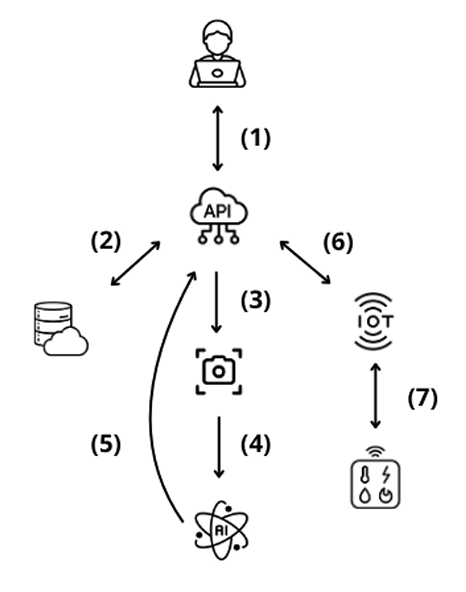
\includegraphics[height=0.65\textheight, keepaspectratio]{imgs/fluxo.png}
    \end{center}
\end{frame}

% ─── APRESENTAÇÃO PRÁTICA ────────────────────────────────────────────────────
\section{Apresentação Prática}

\begin{frame}[b]{Apresentação Prática}
  \begin{columns}[T]
    \begin{column}{0.55\textwidth}
      \begin{itemize}
        \item \textbf{Demonstração} ao vivo do sistema
        \item Principais \textbf{funcionalidades} implementadas
        \item \textbf{Interface} e experiência do usuário
        \item Fluxos de \textbf{uso} e navegação
        \item Casos de uso e \textbf{cenários} práticos
      \end{itemize}
    \end{column}
    \begin{column}{0.40\textwidth}
      \begin{block}{\centering O que será exibido}
        \vspace{0.2em}
        {\scriptsize Sistema MiteScan em execução, com detecção de ácaro, alertas e dashboard de monitoramento.}
        \vspace{0.2em}
      \end{block}
    \end{column}
  \end{columns}
  \vfill
\end{frame}

% ─── RESULTADOS E DISCUSSÕES ─────────────────────────────────────────────────
\section{Resultados e Discussões}

\begin{frame}[b]{Resultados e Discussões}
  \begin{columns}[T]
    \begin{column}{0.55\textwidth}
      \begin{itemize}
        \item O modelo atingiu \textbf{81\%} de acurácia no treinamento e \textbf{62\%} na validação
        \item A classe \textit{normal} teve o melhor resultado, enquanto \textit{varroa} e \textit{asa deformada} apresentaram maior confusão devido à semelhança visual
        \item Os resultados indicam que a ferramenta tem potencial
      \end{itemize}
    \end{column}
    \begin{column}{0.38\textwidth}
      \begin{block}{\centering Acurácia do Modelo}
        \centering
        \vspace{0.4em}
        {\Large\textbf{81\%}}\par
        {\scriptsize Treinamento}\\[0.5em]
        {\large\textbf{62\%}}\par
        {\scriptsize Validação}
        \vspace{0.4em}
      \end{block}
    \end{column}
  \end{columns}
  \vfill
\end{frame}

% ─── SLIDE FINAL (original) ──────────────────────────────────────────────────
{
\usebackgroundtemplate{%
  
\includegraphics[width=\paperwidth,height=\paperheight]{imgs/img_022.jpg}%
}
\begin{frame}[b]{}
  \vspace{0.2cm}
  
  \hspace*{0.25\paperwidth}{\Large \textbf{Obrigado!}}
  
  \vfill
\end{frame}
}

\end{document}